% =====================================================================
%  PROPUESTA DE PROYECTO FINAL DE CARRERA -- Formato paper, 2 columnas
%  Estructura exigida por la rubrica de "Evaluacion - Propuesta PFC":
%    1) Problema computacional a resolver, alcance
%    2) Diseno de proyecto (con Diagrama de Diseno de Proyecto)
%    3) Objetivos (general y especificos): herramientas y alcance
%    4) Resultados esperados
%  Objetivo: 2 hojas. Compilar:  pdflatex propuesta_tesis.tex  (x2)
% =====================================================================
\documentclass[9.5pt,twocolumn,a4paper]{article}
\usepackage[utf8]{inputenc}
\usepackage[T1]{fontenc}
\usepackage{times}
\usepackage[a4paper,top=1.5cm,bottom=1.5cm,left=1.4cm,right=1.4cm,columnsep=0.55cm]{geometry}
\usepackage{amsmath,amssymb}
\usepackage{microtype}
\usepackage[font=small,labelfont=bf,skip=2pt]{caption}
\usepackage{tikz}
\usetikzlibrary{arrows.meta,positioning,fit,calc,backgrounds}
\usepackage{graphicx}
\usepackage[hidelinks]{hyperref}
\usepackage{enumitem}
\setlist{nosep,leftmargin=1.1em}

\setcounter{topnumber}{4}
\setcounter{totalnumber}{6}
\renewcommand{\topfraction}{0.98}
\renewcommand{\textfraction}{0.02}
\renewcommand{\floatpagefraction}{0.90}
\setcounter{dbltopnumber}{4}
\renewcommand{\dbltopfraction}{0.98}
\renewcommand{\dblfloatpagefraction}{0.90}

\setlength{\parindent}{1.0em}
\setlength{\abovedisplayskip}{3pt}
\setlength{\belowdisplayskip}{3pt}
\setlength{\intextsep}{4pt}
\setlength{\textfloatsep}{5pt}
\setlength{\dbltextfloatsep}{5pt}
\setlength{\floatsep}{4pt}

\usepackage{titlesec}
\titlespacing*{\section}{0pt}{5pt}{2pt}
\titleformat{\section}{\normalfont\bfseries}{\thesection}{0.5em}{}

\definecolor{cbase}{HTML}{E8EDF2}
\definecolor{cdata}{HTML}{D6E4F0}
\definecolor{cnew}{HTML}{FFE0B2}
\definecolor{cold}{HTML}{EDEDED}
\definecolor{cout}{HTML}{D9EAD3}
\definecolor{caccent}{HTML}{C05621}

\tikzset{
  blk/.style={rectangle, rounded corners=2pt, draw=black!55, fill=cbase,
              align=center, font=\tiny, minimum height=0.85cm,
              text width=2.8cm, inner sep=3pt},
  dat/.style={blk, fill=cdata},
  new/.style={blk, fill=cnew, draw=caccent, line width=1pt},
  old/.style={blk, fill=cold, draw=black!30, dashed, text=black!45},
  fin/.style={blk, fill=cout},
  op/.style={circle, draw=black!60, fill=white, inner sep=1.5pt, font=\scriptsize},
  fl/.style={-{Latex[length=1.8mm]}, draw=black!65, line width=0.6pt},
  flo/.style={-{Latex[length=1.8mm]}, draw=black!30, dashed, line width=0.6pt},
  flr/.style={-{Latex[length=2.4mm]}, draw=caccent, line width=1.1pt},
  lbl/.style={font=\tiny\itshape, text=black!60, align=center},
  col/.style={blk, text width=3.6cm, minimum height=1.1cm}
}

% --- paleta y estilos para el "Diagrama de diseño teórico" (Fig. 2), en
%     tonos de plomo/gris, con prefijo td- para no chocar con los estilos de
%     arriba ---
\definecolor{gdata}{HTML}{94A3B8}
\definecolor{gdatabg}{HTML}{F4F6F8}
\definecolor{gcomp}{HTML}{64748B}
\definecolor{gcompbg}{HTML}{F1F3F5}
\definecolor{gtec}{HTML}{1E293B}
\definecolor{gtecbg}{HTML}{ECEDF0}
\definecolor{gval}{HTML}{475569}
\definecolor{gvalbg}{HTML}{F0F2F4}
\definecolor{gzone}{HTML}{FAFAFB}
\definecolor{gzb}{HTML}{D9DBDF}
\definecolor{garrow}{HTML}{3F3F46}
\tikzset{
  tdzone/.style={rectangle, rounded corners=8pt, draw=gzb, fill=gzone, line width=0.7pt},
  tdlbl/.style={font=\bfseries\small, draw=gzb, fill=white, rounded corners=2pt,
               inner sep=3pt, text=black!70},
  tdcard/.style={rectangle, rounded corners=5pt, align=left, font=\scriptsize,
              text width=3.3cm, inner sep=7pt, line width=1.2pt},
  tdfl/.style={-{Latex[length=2.4mm]}, draw=garrow, line width=1.0pt},
  tdflh/.style={-{Latex[length=2.6mm]}, draw=gtec, line width=1.7pt},
  tdleg/.style={rectangle, rounded corners=1.5pt, minimum width=3.2mm, minimum height=3.2mm}
}

% --- paleta y estilos para el "Diagrama de flujo general" (Fig. 3) ---
\definecolor{f1}{HTML}{CBD5E1}
\definecolor{f1bg}{HTML}{F4F6F8}
\definecolor{f2}{HTML}{94A3B8}
\definecolor{f2bg}{HTML}{EEF1F4}
\definecolor{f3}{HTML}{64748B}
\definecolor{f3bg}{HTML}{E9ECEF}
\definecolor{f4}{HTML}{334155}
\definecolor{f4bg}{HTML}{E4E7EB}
\definecolor{f5}{HTML}{1E293B}
\definecolor{f5bg}{HTML}{DFE3E7}
\definecolor{farrow}{HTML}{3F3F46}
\tikzset{
  fstep/.style={rectangle, rounded corners=6pt, align=center, font=\scriptsize,
               text width=2.55cm, minimum height=2.1cm, inner sep=6pt, line width=1.2pt},
  ffl/.style={-{Latex[length=2.6mm]}, draw=farrow, line width=1.3pt}
}

\begin{document}
\pagestyle{empty}

\twocolumn[
\begin{center}
{\Large\bfseries Representaciones auto-supervisadas para el descubrimiento de
clases novedosas en segmentación semántica de nubes de puntos 3D\par}
\vspace{4pt}
{\normalsize Renzo [Apellido] \quad Manyory Cueva Mendoza\par}
\vspace{2pt}
{\small Escuela Profesional de Ingeniería de Sistemas / Ciencia de la
Computación\par}
\vspace{1pt}
{\small\itshape Propuesta de Proyecto Final de Carrera --- \today\par}
\end{center}
\vspace{3pt}
\begin{quotation}
\noindent\small\textbf{Resumen.}
La segmentación semántica de nubes de puntos opera bajo un supuesto de
conjunto cerrado: todo punto se asigna forzosamente a una clase conocida. El
paradigma \emph{Novel Class Discovery} (NCD) levanta ese supuesto, pero su
estado del arte en 3D ---HyperNCD~\cite{hyperncd}, 2026--- alcanza apenas
11.8--47.5 mIoU en clases novedosas frente a 49.8 del modelo supervisado en
SemanticKITTI. Identificamos una causa plausible: HyperNCD construye sus
prototipos con descriptores geométricos manuales (linealidad, planaridad,
\emph{scattering}). Sonata~\cite{sonata} demostró que apoyarse en señales
geométricas de bajo nivel induce el \emph{geometric shortcut}, un colapso
representacional que impide aprender semántica, y que corregirlo eleva el
\emph{linear probing} de 21.8\,\% a 72.5\,\% mIoU en ScanNet. Ningún trabajo ha
trasladado ese hallazgo a NCD. Proponemos sustituir el bloque geométrico
manual de HyperNCD por el \emph{encoder} auto-supervisado de Sonata, congelado,
y medir el efecto en SemanticKITTI y SemanticPOSS.
\vspace{2pt}

\noindent\small\textbf{Palabras clave:} nubes de puntos, segmentación semántica
3D, \emph{novel class discovery}, aprendizaje auto-supervisado, hipergrafos.
\end{quotation}
\vspace{4pt}
]

% ---------------------------------------------------------------------
\section{Problema computacional y alcance}
% ---------------------------------------------------------------------
Partimos de nubes de puntos 3D ya capturadas y etiquetadas,
$P=\{(x_i,f_i)\}_{i=1}^{N}$, provistas por los conjuntos de datos
SemanticKITTI y SemanticPOSS; no se procesa señal cruda de sensor alguno,
solo los \emph{datasets} públicos. La
segmentación semántica asigna una etiqueta $y_i$ a cada punto. Los métodos
actuales resuelven bien la tarea ---PTv3~\cite{ptv3}: 77.5 mIoU; Sonata:
79.4 mIoU en ScanNet--- pero comparten una restricción: \emph{el conjunto de
clases está cerrado en entrenamiento}. Un objeto no previsto no se marca como
«desconocido»: se fuerza a la clase conocida más cercana, un modo de falla
silencioso en conducción autónoma o robótica móvil.

\emph{Novel Class Discovery} (NCD), introducido a nubes de puntos por Riz
\emph{et al.}~\cite{nops}, formaliza el problema: dado $\mathcal{C}_k$
(clases conocidas, etiquetadas) y $\mathcal{C}_n$ (novedosas, sin etiqueta),
el modelo debe segmentar ambas. El estado del arte, HyperNCD~\cite{hyperncd},
modela asociaciones de alto orden vía un hipergrafo de \emph{prototipos
geométrico-conscientes}: cada punto se representa como
$F_i=[f_{\mathrm{sem}}(x^i);f_{\mathrm{geo}}(x^i)]$, donde $f_{\mathrm{geo}}$
se calcula analíticamente (linealidad, planaridad, \emph{scattering} sobre
$k$NN, $k{=}15$).

Sonata~\cite{sonata} identifica el \emph{geometric shortcut}: el modelo
colapsa sobre pistas geométricas accesibles (normales, altura) en vez de
aprender semántica; con \emph{linear probing} lo cuantifica: PointContrast
5.6\,\%, MSC 21.8\,\%, Sonata 72.5\,\% mIoU en ScanNet. HyperNCD (jun.\ 2026)
es posterior a Sonata (mar.\ 2025) pero construye su módulo central sobre el
tipo de descriptor que Sonata caracteriza como problemático, sin citarlo
---los dos trabajos nunca se han conectado porque atacan problemas distintos.
Hipótesis:

\begin{quotation}\noindent\footnotesize\itshape
Si $f_{\mathrm{geo}}$ se reemplaza por embeddings de un \emph{encoder}
auto-supervisado congelado, los prototipos serán más discriminativos y
mejorará el mIoU en clases novedosas.
\end{quotation}

\textbf{Incluye:} SemanticKITTI (sec.\ 08) y SemanticPOSS (sec.\ 03), 4
\emph{splits} oficiales~\cite{nops,dasl}; \emph{encoder} congelado;
comparación contra NOPS, DASL, HyperNCD; ablación.
\textbf{Excluye:} preentrenamiento SSL propio (Sonata: 140k escenas, 32 GPU);
detección/instancias; vocabulario abierto basado en LLM; tiempo real embebido.

% ---------------------------------------------------------------------
\section{Diseño de proyecto}
% ---------------------------------------------------------------------
La Fig.~\ref{fig:teorico} es el \textbf{diagrama de diseño de proyecto}: ubica
el punto de intervención sobre la arquitectura de HyperNCD y a qué objetivo
específico corresponde cada módulo. El \emph{encoder} de Sonata reemplaza la
rama geométrica manual, antes de la concatenación. Todo lo posterior de
HyperNCD ---prototipos por \texttt{Conv1d}+\emph{softmax},
$R_k=\sum_i s_{i,k}(F^i_r-P_k)$, hipergrafo con $M{=}8$ vecinos, ajuste
dinámico y pseudo-etiquetas--- se mantiene intacto. Al mover una sola pieza,
cualquier cambio en las métricas es atribuible al reemplazo, lo que hace la
ablación interpretable sin ambigüedad.

\textbf{Notación.} $f_{\mathrm{sem}}$ y $f_{\mathrm{ssl}}$ son los
descriptores por punto que produce cada rama: el semántico
(\emph{backbone} MinkowskiUNet-34C, ya en HyperNCD) y el auto-supervisado
(\emph{encoder} Sonata, congelado). Ambos se concatenan en
$F_i=[f_{\mathrm{sem}}(x^i);f_{\mathrm{ssl}}(x^i)]$ ---la Ec.~3 de HyperNCD
con $f_{\mathrm{geo}}$ reemplazado por $f_{\mathrm{ssl}}$--- para formar cada
prototipo. La afinidad entre dos prototipos combina una componente
geométrica $S_g$ y una semántica $S_s$ mediante
$S_b=\alpha S_g+(1-\alpha)S_s$ (Ec.~6 de HyperNCD), donde $\alpha\in[0,1]$
pondera ambas; $S_b$ decide, para cada prototipo, sus $M{=}8$ vecinos más
afines al construir el hipergrafo.

\begin{figure*}[t]
\centering
\vspace{-6pt}
\resizebox{0.92\textwidth}{!}{%
\begin{tikzpicture}[font=\sffamily]

\node[tdcard, draw=gdata, fill=gdatabg] (m0) at (0,0)
 {\textbf{M0: Adquisición y Preprocesamiento}\\[2pt]
  {\itshape\footnotesize\color{gdata!60!black}(Ciencia de Datos)}\\[3pt]
  \textbullet\ SemanticKITTI · SemanticPOSS (4 \emph{splits})\\
  \textbullet\ MinkowskiEngine: voxelización y normalización};

\node[tdcard, draw=gcomp, fill=gcompbg] (m1) at (4.6,2.35)
 {\textbf{M1: Extracción de Características}\\[2pt]
  {\itshape\footnotesize\color{gcomp!60!black}(IA y Aprendizaje Automático)}\\[3pt]
  \textbullet\ MinkowskiUNet-34C $\rightarrow f_{\mathrm{sem}}(x^i)$};

\node[tdcard, draw=gtec, fill=gtecbg] (m2) at (4.6,-2.35)
 {\textbf{M2: Encoder Auto-supervisado (Sonata)}\\[2pt]
  {\itshape\footnotesize\color{gtec}(Técnica Complementaria --- APORTE)}\\[3pt]
  \textbullet\ PTv3 congelado (Pointcept) $\rightarrow f_{\mathrm{ssl}}(x^i)$\\
  \textbullet\ reemplaza $f_{\mathrm{geo}}$ (OE2)};

\node[tdcard, draw=gcomp, fill=gcompbg] (m3) at (9.3,0)
 {\textbf{M3: Prototipos y Razonamiento por Hipergrafo}\\[2pt]
  {\itshape\footnotesize\color{gcomp!60!black}(IA y Aprendizaje Automático)}\\[3pt]
  \textbullet\ $F_i=[f_{\mathrm{sem}};f_{\mathrm{ssl}}]$, Conv1d+\emph{softmax}\\
  \textbullet\ $S_b=\alpha S_g+(1-\alpha)S_s,\ M{=}8$};

\node[tdcard, draw=gval, fill=gvalbg] (m4) at (13.3,0)
 {\textbf{M4: Evaluación y Comparación}\\[2pt]
  {\itshape\footnotesize\color{gval}(Validación)}\\[3pt]
  \textbullet\ mIoU húngaro vs.\ NOPS · DASL · HyperNCD\\
  \textbullet\ criterio: $\geq$2/4 \emph{splits}, sin degradar \emph{known}};

\begin{pgfonlayer}{background}
\node[tdzone, fit=(m0), inner xsep=16pt, inner ysep=16pt] (zE) {};
\node[tdzone, fit=(m1)(m2)(m3), inner xsep=16pt, inner ysep=16pt] (zP) {};
\node[tdzone, fit=(m4), inner xsep=16pt, inner ysep=16pt] (zS) {};
\end{pgfonlayer}

\node[tdlbl, anchor=south] (lblE) at ($(zE.north)+(0,0.10)$) {ENTRADA};
\node[tdlbl, anchor=south] (lblP) at ($(zP.north)+(0,0.10)$) {PROCESO};
\node[tdlbl, anchor=south] (lblS) at ($(zS.north)+(0,0.10)$) {SALIDA};

\node[tdleg, fill=gdata, anchor=west] (lg1) at ($(lblP.north)+(-2.6,0.55)$) {};
\node[anchor=west, font=\scriptsize] at ($(lg1.east)+(0.12,0)$) {Ciencia de Datos};
\node[tdleg, fill=gcomp, anchor=west] (lg2) at ($(lblP.north)+(1.6,0.55)$) {};
\node[anchor=west, font=\scriptsize] at ($(lg2.east)+(0.12,0)$) {IA y Aprendizaje Automático};
\node[tdleg, fill=gtec, anchor=west] (lg3) at ($(lblP.north)+(-2.6,0.15)$) {};
\node[anchor=west, font=\scriptsize] at ($(lg3.east)+(0.12,0)$) {Técnica Complementaria};
\node[tdleg, fill=gval, anchor=west] (lg4) at ($(lblP.north)+(1.6,0.15)$) {};
\node[anchor=west, font=\scriptsize] at ($(lg4.east)+(0.12,0)$) {Validación};

\draw[tdfl] (m0.east) -- (m1.west);
\draw[tdfl] (m0.east) -- (m2.west);
\draw[tdfl] (m1.east) -- (m3.north west);
\draw[tdflh] (m2.east) -- (m3.south west);
\node[font=\tiny\itshape, text=gtec, align=center]
  at ($(m2.east)!0.5!(m3.south west)+(0,-0.45)$) {integración (OE2)};
\draw[tdfl] (m3.east) -- (m4.west);

\end{tikzpicture}}
\vspace{-4pt}
\caption{\textbf{Diagrama de diseño teórico, por módulos.} Relación
entrada--proceso--salida: M0 adquiere y preprocesa las nubes de puntos; M1 y
M3 (\emph{Área de Computación}) reproducen la maquinaria original de HyperNCD
sin modificar; M2 es la técnica complementaria --el \emph{encoder} SSL de
Sonata, congelado-- que constituye el aporte de la tesis (OE2) y se integra a
M3 en reemplazo del bloque geométrico manual; M4 evalúa y compara contra el
estado del arte.}
\label{fig:teorico}
\vspace{-6pt}
\end{figure*}

El criterio de éxito se fija sobre \textbf{mIoU de clases novedosas} tras
emparejamiento húngaro: mejora sobre HyperNCD en $\geq$2 de 4 \emph{splits},
sin degradar clases conocidas (Fig.~\ref{fig:teorico}).

\textbf{Riesgo y mitigación.} Sonata se preentrenó mayoritariamente en
interiores densos; en exteriores su \emph{linear probing} en SemanticKITTI
(62.0 mIoU) queda por debajo de PTv3 entrenado desde cero (69.1), y 2.9
puntos por debajo fuera de distribución. \emph{Plan B:} concatenar en vez de
sustituir, $F_i=[f_{\mathrm{sem}};f_{\mathrm{geo}};f_{\mathrm{ssl}}]$, dejando
que el módulo de prototipos pondere. Cualquier resultado ---mejora, paridad o
degradación--- documentado con ablación es un hallazgo reportable.

\textbf{Marco metodológico.} La Fig.~\ref{fig:flujo} complementa el diagrama
anterior con la secuencia operativa de principio a fin: carga de la nube de
puntos, preparación del \emph{input}, filtrado (Módulo 1), segmentación
semántica con prototipos e hipergrafo (Módulo 2, donde se integra
$f_{\mathrm{ssl}}$) y evaluación comparativa (Módulo 3).

% ============ FIGURA: DIAGRAMA DE FLUJO GENERAL ==============
\begin{figure*}[t]
\centering
\vspace{-4pt}
\resizebox{0.97\textwidth}{!}{%
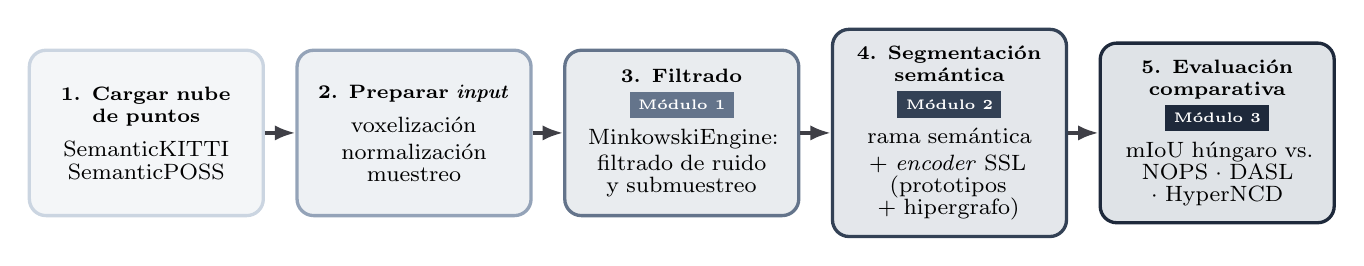
\begin{tikzpicture}[font=\sffamily]

\node[fstep, draw=f1, fill=f1bg] (s1) at (0,0)
 {\textbf{1. Cargar nube de puntos}\\[3pt]
  {\footnotesize SemanticKITTI \\ SemanticPOSS}};

\node[fstep, draw=f2, fill=f2bg] (s2) at (3.4,0)
 {\textbf{2. Preparar \emph{input}}\\[3pt]
  {\footnotesize voxelización\\normalización\\muestreo}};

\node[fstep, draw=f3, fill=f3bg] (s3) at (6.8,0)
 {\textbf{3. Filtrado}\\[2pt]
  \colorbox{f3}{\textcolor{white}{\textbf{\tiny Módulo 1}}}\\[3pt]
  {\footnotesize MinkowskiEngine:\\filtrado de ruido\\y submuestreo}};

\node[fstep, draw=f4, fill=f4bg, text=black] (s4) at (10.2,0)
 {\textbf{4. Segmentación semántica}\\[2pt]
  \colorbox{f4}{\textcolor{white}{\textbf{\tiny Módulo 2}}}\\[3pt]
  {\footnotesize rama semántica\\$+$ \emph{encoder} SSL\\(prototipos $+$ hipergrafo)}};

\node[fstep, draw=f5, fill=f5bg] (s5) at (13.6,0)
 {\textbf{5. Evaluación comparativa}\\[2pt]
  \colorbox{f5}{\textcolor{white}{\textbf{\tiny Módulo 3}}}\\[3pt]
  {\footnotesize mIoU húngaro vs.\\NOPS $\cdot$ DASL $\cdot$ HyperNCD}};

\draw[ffl] (s1.east) -- (s2.west);
\draw[ffl] (s2.east) -- (s3.west);
\draw[ffl] (s3.east) -- (s4.west);
\draw[ffl] (s4.east) -- (s5.west);

\end{tikzpicture}}
\vspace{-4pt}
\caption{\textbf{Diagrama de flujo general (marco metodológico).} Secuencia
operativa desde la carga de datos hasta la evaluación; los módulos 1--3
corresponden a las etapas de filtrado, segmentación (con la integración
$F_i=[f_{\mathrm{sem}};f_{\mathrm{ssl}}]$) y comparación de la
Fig.~\ref{fig:teorico}.}
\label{fig:flujo}
\vspace{-8pt}
\end{figure*}











% ---------------------------------------------------------------------
\section{Objetivos del proyecto}
% ---------------------------------------------------------------------
\textbf{General.} Diseñar y evaluar un método de descubrimiento de clases
novedosas para segmentación 3D que sustituya los descriptores geométricos
manuales por representaciones auto-supervisadas preentrenadas, midiendo su
impacto en SemanticKITTI y SemanticPOSS.

\textbf{OE1 (Reproducir el estado del arte).} Replicar HyperNCD en ambos
datasets, 4 \emph{splits} oficiales, con desviación reportada sobre 3
corridas. \emph{Herramientas:} Python 3.10, PyTorch, MinkowskiEngine, código
oficial de HyperNCD, MinkowskiUNet-34C. \emph{Alcance:} desviación
$\pm1.0$ mIoU respecto de lo publicado.

\textbf{OE2 (Integrar el \emph{encoder} SSL).} Incorporar el \emph{encoder}
de Sonata (pesos congelados, \emph{up-cast}) en el módulo de prototipos, en
reemplazo del bloque geométrico analítico. \emph{Herramientas:} pesos
públicos de Sonata, Pointcept, PTv3, \texttt{spconv}. \emph{Alcance:} solo
inferencia, sin retropropagación a través del \emph{encoder}.

\textbf{OE3 (Reajustar la configuración).} Recalibrar $\alpha$ (balance
geométrico-semántico), $M$ (vecinos por hiperarista) y $\epsilon$ (suavizado
de etiquetas). \emph{Herramientas:} Optuna/grilla, AdamW, Weights\&Biases.
\emph{Alcance:} búsqueda en \emph{split} 0, aplicada sin reajuste a los otros
tres.

\textbf{OE4 (Evaluar y ablacionar).} Comparar contra NOPS~\cite{nops},
DASL~\cite{dasl} e HyperNCD en mIoU \emph{novel}/\emph{known}/\emph{all};
ablación que aísla la contribución del \emph{encoder} (manual /
auto-supervisado / concatenación). \emph{Herramientas:} mIoU con
emparejamiento húngaro, visualizaciones PCA. \emph{Alcance:} 4 \emph{splits}
por dataset, sin evaluación en interiores.

\emph{Recursos:} GPU de gama media (VRAM $\geq$12\,GB); el \emph{encoder}
congelado solo añade costo de inferencia (\emph{cache} de características por
escena). Respaldo: Colab Pro / Kaggle, con OE3 reducido a grilla acotada si
aplica.

% ---------------------------------------------------------------------
\section{Resultados esperados}
% ---------------------------------------------------------------------
Se espera una mejora del mIoU en clases novedosas sobre HyperNCD en al menos
2 de los 4 \emph{splits} de SemanticKITTI y SemanticPOSS, sin degradación de
las clases conocidas ---el criterio de éxito fijado en la Fig.~\ref{fig:teorico}.
Como entregables intermedios: (i) tabla de reproducción de HyperNCD con
desviación reportada (OE1); (ii) implementación integrada y repositorio
público del \emph{encoder} SSL dentro del módulo de prototipos (OE2); (iii)
curvas de sensibilidad de $\alpha$, $M$ y $\epsilon$ (OE3); (iv) tablas
comparativas contra NOPS, DASL y HyperNCD, y estudio de ablación que aísla la
contribución del \emph{encoder} congelado (OE4).

La contribución no es una arquitectura nueva, sino establecer empíricamente
si un hallazgo demostrado en régimen supervisado ---la nocividad del
\emph{geometric shortcut}--- se transfiere a un régimen sin supervisión sobre
las clases objetivo, donde la calidad de la representación es más crítica.
Bajo el Plan B (Sec.~2), incluso un resultado nulo o negativo, documentado
con ablación, constituye un hallazgo reportable: es un resultado incierto y
medible, condición que justifica investigarlo.

{\small
\begin{thebibliography}{9}
\bibitem{nops} L. Riz, C. Saltori, E. Ricci, F. Poiesi, «Novel Class
Discovery for 3D Point Cloud Semantic Segmentation», \emph{CVPR}, 2023.
\bibitem{ptv3} X. Wu \emph{et al.}, «Point Transformer V3: Simpler, Faster,
Stronger», \emph{CVPR}, 2024.
\bibitem{dasl} R. Xu, C. Zhang, H. Ren, X. He, «Dual-Level Adaptive
Self-Labeling for Novel Class Discovery in Point Cloud Segmentation»,
\emph{ECCV}, 2024.
\bibitem{sonata} X. Wu \emph{et al.}, «Sonata: Self-Supervised Learning of
Reliable Point Representations», \emph{arXiv:2503.16429}, 2025.
\bibitem{hyperncd} Z. Zhang, A. Wu, Y. Li, Y. Han, J. Shen, «Geometric-Aware
Hypergraph Reasoning for Novel Class Discovery in Point Cloud Segmentation»,
\emph{arXiv:2606.07280}, 2026.
\end{thebibliography}}




% ============================================================
% DIAGRAMA DE DISEÑO DEL SISTEMA
% Pegar dentro del documento, antes de Objetivos del proyecto
% ============================================================

\begin{figure*}[t]
\centering
\vspace{-3pt}

\resizebox{0.98\textwidth}{!}{%
\begin{tikzpicture}[
    font=\sffamily,

    module/.style={
        rectangle,
        rounded corners=7pt,
        fill=white,
        line width=1.1pt,
        minimum width=3.25cm,
        minimum height=6.25cm
    },

    groupblue/.style={
        rectangle,
        rounded corners=11pt,
        draw=blue!75!black,
        fill=blue!2,
        dashed,
        line width=1pt
    },

    groupcyan/.style={
        rectangle,
        rounded corners=11pt,
        draw=cyan!65!black,
        fill=cyan!2,
        dashed,
        line width=1pt
    },

    groupgreen/.style={
        rectangle,
        rounded corners=11pt,
        draw=green!55!black,
        fill=green!2,
        dashed,
        line width=1pt
    },

    grouporange/.style={
        rectangle,
        rounded corners=11pt,
        draw=orange!85!black,
        fill=orange!2,
        dashed,
        line width=1pt
    },

    header/.style={
        rectangle,
        rounded corners=4pt,
        text=white,
        font=\bfseries\footnotesize,
        inner xsep=9pt,
        inner ysep=5pt
    },

    cardtitle/.style={
        font=\bfseries\small,
        align=center,
        text=black!88
    },

    subtitle/.style={
        font=\scriptsize,
        align=center,
        text width=2.75cm,
        text=black!80
    },

    infobox/.style={
        rectangle,
        rounded corners=5pt,
        align=left,
        text width=2.72cm,
        inner sep=7pt,
        font=\tiny,
        line width=0.8pt
    },

    flow/.style={
        -{Latex[length=3mm,width=2mm]},
        draw=black!80,
        line width=1.4pt
    }
]

% ============================================================
% TÍTULO
% ============================================================

\node[
    font=\bfseries\Large,
    text=black!85
] at (6.45,4.25)
{Diagrama de diseño del sistema propuesto};

% ============================================================
% TARJETAS PRINCIPALES
% ============================================================

\node[
    module,
    draw=blue!75!black
] (entrada) at (0,0) {};

\node[
    module,
    draw=cyan!65!black
] (proceso) at (4.30,0) {};

\node[
    module,
    draw=green!55!black
] (modelo) at (8.60,0) {};

\node[
    module,
    draw=orange!85!black
] (salida) at (12.90,0) {};

% ============================================================
% CONTENEDORES EXTERNOS
% ============================================================

\begin{pgfonlayer}{background}

\node[
    groupblue,
    fit=(entrada),
    inner xsep=7pt,
    inner ysep=9pt
] (gentrada) {};

\node[
    groupcyan,
    fit=(proceso),
    inner xsep=7pt,
    inner ysep=9pt
] (gproceso) {};

\node[
    groupgreen,
    fit=(modelo),
    inner xsep=7pt,
    inner ysep=9pt
] (gmodelo) {};

\node[
    grouporange,
    fit=(salida),
    inner xsep=7pt,
    inner ysep=9pt
] (gsalida) {};

\end{pgfonlayer}

% ============================================================
% ENCABEZADOS
% ============================================================

\node[
    header,
    fill=blue!75!black
] at (gentrada.north)
{MÓDULO 1: ENTRADA};

\node[
    header,
    fill=cyan!65!black
] at (gproceso.north)
{MÓDULO 2: PROCESAMIENTO};

\node[
    header,
    fill=green!55!black
] at (gmodelo.north)
{MÓDULO 3: MODELO};

\node[
    header,
    fill=orange!85!black
] at (gsalida.north)
{MÓDULO 4: SALIDA};

% ============================================================
% MÓDULO 1: ÍCONO DE NUBE DE PUNTOS
% ============================================================

\begin{scope}[
    shift={($(entrada.north)+(0,-1.20)$)},
    scale=0.54
]

\draw[
    blue!70!black,
    line width=0.8pt
]
(-1.35,-0.50) --
(0,-1.25) --
(1.35,-0.50) --
(1.35,0.65) --
(0,1.40) --
(-1.35,0.65) -- cycle;

\draw[blue!45, line width=0.6pt]
(0,-1.25) -- (0,0.05) -- (1.35,0.65);

\draw[blue!45, line width=0.6pt]
(0,0.05) -- (-1.35,0.65);

\draw[blue!45, line width=0.6pt]
(0,0.05) -- (0,1.40);

\foreach \x/\y in {
-1.15/-0.30,-0.95/-0.42,-0.72/-0.55,
-0.48/-0.70,-0.23/-0.86,
0.23/-0.86,0.48/-0.70,0.72/-0.55,
0.95/-0.42,1.15/-0.30,
-1.02/0.08,-0.76/0.22,-0.50/0.36,
-0.24/0.50,0/0.64,
0.24/0.50,0.50/0.36,0.76/0.22,1.02/0.08,
-0.70/0.68,-0.45/0.83,-0.20/0.98,
0/1.10,0.20/0.98,0.45/0.83,0.70/0.68
}{
    \fill[blue!75!black] (\x,\y) circle (1.6pt);
}

\foreach \x/\h in {
-0.75/0.70,
-0.30/0.95,
0.20/0.72,
0.68/0.90
}{
    \draw[
        blue!70!black,
        densely dotted,
        line width=1pt
    ] (\x,-0.15) -- (\x,\h);
}

\end{scope}

\node[
    cardtitle
] at ($(entrada.center)+(0,0.72)$)
{Datos de entrada};

\node[
    subtitle
] at ($(entrada.center)+(0,0.08)$)
{Nubes de puntos 3D\\
SemanticKITTI y SemanticPOSS};

\node[
    infobox,
    draw=blue!55,
    fill=blue!5
] at ($(entrada.center)+(0,-1.65)$)
{
\textbullet\ Coordenadas $(x,y,z)$\\[4pt]
\textbullet\ Intensidad o reflectancia\\[4pt]
\textbullet\ Clases conocidas etiquetadas\\[4pt]
\textbullet\ Clases novedosas sin etiqueta\\[4pt]
\textbullet\ Cuatro \emph{splits} oficiales
};

% ============================================================
% MÓDULO 2: ÍCONO DE PREPROCESAMIENTO
% ============================================================

\begin{scope}[
    shift={($(proceso.north)+(0,-1.18)$)},
    scale=0.57
]

\foreach \x/\y in {
-0.70/1.10,
0/1.10,
0.70/1.10,
-0.43/0.68,
0.18/0.68,
0.76/0.68
}{
    \fill[cyan!65!black] (\x,\y) circle (4pt);
}

\filldraw[
    fill=cyan!70,
    draw=cyan!65!black,
    line width=0.8pt
]
(-1.15,0.28) --
(1.15,0.28) --
(0.45,-0.48) --
(0.45,-1.02) --
(0.14,-1.30) --
(-0.14,-1.30) --
(-0.45,-1.02) --
(-0.45,-0.48) -- cycle;

\fill[cyan!65!black] (-0.25,-1.62) circle (3.4pt);
\fill[cyan!65!black] (0.25,-1.62) circle (3.4pt);

\end{scope}

\node[
    cardtitle
] at ($(proceso.center)+(0,0.72)$)
{Preparación del \emph{input}};

\node[
    subtitle
] at ($(proceso.center)+(0,0.08)$)
{Transformación de la nube para\\
el procesamiento computacional};

\node[
    infobox,
    draw=cyan!55!black,
    fill=cyan!5
] at ($(proceso.center)+(0,-1.65)$)
{
\textbullet\ Voxelización\\[4pt]
\textbullet\ Normalización\\[4pt]
\textbullet\ Muestreo y organización\\[4pt]
\textbullet\ MinkowskiEngine\\[4pt]
\textbullet\ Separación \emph{known}/\emph{novel}
};

% ============================================================
% MÓDULO 3: ÍCONO DEL MODELO
% ============================================================

\begin{scope}[
    shift={($(modelo.north)+(0,-1.16)$)},
    scale=0.55
]

\foreach \ya in {0.85,0,-0.85}{
    \foreach \yb in {1.10,0.36,-0.36,-1.10}{
        \draw[
            green!45!black,
            line width=0.55pt
        ] (-1.25,\ya) -- (0,\yb);
    }
}

\foreach \yb in {1.10,0.36,-0.36,-1.10}{
    \draw[
        green!45!black,
        line width=0.55pt
    ] (0,\yb) -- (1.35,0);
}

\foreach \y in {0.85,0,-0.85}{
    \filldraw[
        fill=white,
        draw=green!55!black,
        line width=1.1pt
    ] (-1.25,\y) circle (0.17);
}

\foreach \y in {1.10,0.36,-0.36,-1.10}{
    \filldraw[
        fill=white,
        draw=green!55!black,
        line width=1.1pt
    ] (0,\y) circle (0.17);
}

\filldraw[
    fill=white,
    draw=green!55!black,
    line width=1.1pt
] (1.35,0) circle (0.17);

\end{scope}

\node[
    cardtitle
] at ($(modelo.center)+(0,0.82)$)
{Segmentación y descubrimiento};

\node[
    subtitle
] at ($(modelo.center)+(0,0.28)$)
{Extracción de características y\\
razonamiento entre clases};

\node[
    rectangle,
    rounded corners=3pt,
    draw=green!55!black,
    fill=green!10,
    text=green!35!black,
    font=\bfseries\tiny,
    inner xsep=5pt,
    inner ysep=3pt
] at ($(modelo.center)+(0,-0.18)$)
{APORTE: ENCODER SONATA};

\node[
    infobox,
    draw=green!55!black,
    fill=green!5
] at ($(modelo.center)+(0,-1.78)$)
{
\textbullet\ MinkowskiUNet-34C:
$f_{\mathrm{sem}}$\\[4pt]

\textbullet\ Sonata/PTv3 congelado:
$f_{\mathrm{ssl}}$\\[4pt]

\textbullet\ Integración:
$F_i=[f_{\mathrm{sem}};f_{\mathrm{ssl}}]$\\[4pt]

\textbullet\ Prototipos por clase\\[4pt]

\textbullet\ Hipergrafo dinámico y pseudo-etiquetas
};

% ============================================================
% MÓDULO 4: ÍCONO DE SEGMENTACIÓN
% ============================================================

\begin{scope}[
    shift={($(salida.north)+(0,-1.18)$)},
    scale=0.57
]

\filldraw[
    fill=blue!60,
    draw=black!70,
    line width=0.6pt
] (-1.35,-0.85) rectangle (-0.45,0.05);

\filldraw[
    fill=green!60,
    draw=black!70,
    line width=0.6pt
] (-0.40,-0.85) rectangle (0.45,0.20);

\filldraw[
    fill=orange!70,
    draw=black!70,
    line width=0.6pt
] (0.50,-0.85) rectangle (1.35,0.15);

\filldraw[
    fill=violet!60,
    draw=black!70,
    line width=0.6pt
] (-1.35,0.10) rectangle (-0.45,1.00);

\filldraw[
    fill=cyan!60,
    draw=black!70,
    line width=0.6pt
] (-0.40,0.25) rectangle (0.45,1.00);

\filldraw[
    fill=red!60,
    draw=black!70,
    line width=0.6pt
] (0.50,0.20) rectangle (1.35,1.00);

\draw[
    black!80,
    line width=1pt
] (-1.40,-0.90) rectangle (1.40,1.05);

\end{scope}

\node[
    cardtitle
] at ($(salida.center)+(0,0.72)$)
{Resultados del sistema};

\node[
    subtitle
] at ($(salida.center)+(0,0.08)$)
{Segmentación por punto de clases\\
conocidas y novedosas};

\node[
    infobox,
    draw=orange!75!black,
    fill=orange!6
] at ($(salida.center)+(0,-1.65)$)
{
\textbullet\ Etiqueta semántica por punto\\[4pt]
\textbullet\ Clases conocidas y novedosas\\[4pt]
\textbullet\ Nube segmentada en 3D\\[4pt]
\textbullet\ mIoU \emph{novel}, \emph{known} y \emph{all}\\[4pt]
\textbullet\ Comparación con NOPS, DASL e HyperNCD
};

% ============================================================
% FLECHAS
% ============================================================

\draw[flow] (gentrada.east) -- (gproceso.west);
\draw[flow] (gproceso.east) -- (gmodelo.west);
\draw[flow] (gmodelo.east) -- (gsalida.west);

\node[
    font=\tiny\itshape,
    fill=white,
    text=black!60,
    inner sep=1pt
] at ($(gentrada.east)!0.5!(gproceso.west)+(0,0.24)$)
{datos};

\node[
    font=\tiny\itshape,
    fill=white,
    text=black!60,
    inner sep=1pt
] at ($(gproceso.east)!0.5!(gmodelo.west)+(0,0.24)$)
{características};

\node[
    font=\tiny\itshape,
    fill=white,
    text=black!60,
    inner sep=1pt
] at ($(gmodelo.east)!0.5!(gsalida.west)+(0,0.24)$)
{predicciones};

\end{tikzpicture}%
}

\vspace{-2pt}

\caption{
\textbf{Diagrama de diseño del sistema propuesto.}
Las nubes de puntos de SemanticKITTI y SemanticPOSS son voxelizadas y
normalizadas antes de ingresar al modelo. MinkowskiUNet-34C obtiene las
características semánticas $f_{\mathrm{sem}}$, mientras que el encoder
auto-supervisado congelado de Sonata produce $f_{\mathrm{ssl}}$.
Las representaciones se integran para construir prototipos y un hipergrafo
dinámico que permite segmentar clases conocidas y descubrir clases novedosas.
}

\label{fig:flujo}

\vspace{-7pt}
\end{figure*}

\end{document}
